\documentclass[10pt,letterpaper,fleqn,titlepage]{article}

% Define packages to use
\usepackage[letterpaper,top=0.85in,bottom=0.75in,left=0.75in,right=0.75in]{geometry}
%\usepackage{natbib}
%\bibliographystyle{plainnat}
\usepackage{graphicx,color}
\usepackage{subcaption}
\usepackage{amsmath,amssymb}
\usepackage{bm}
\usepackage{caption}
\usepackage{xr}
\usepackage{ifthen}
\usepackage[colorlinks,linkcolor=blue,citecolor=blue,urlcolor=blue]{hyperref}
\usepackage{fancybox}
\usepackage{textcomp}
\usepackage{fancyhdr}
\usepackage{alltt}
\usepackage{float}
\usepackage{svn}
\usepackage{longtable}
\usepackage{array}


% Some new columntypes to allow fixed widths but
% with alignment the same as the regular c,l,r
% (requires array package). An example:
%   \begin{tabular}{C{2cm} *{3}{R{1cm}@{.}L{2cm}}}
\newcolumntype{C}[1]{>{\centering\arraybackslash}p{#1}}
\newcolumntype{L}[1]{>{\raggedright\arraybackslash}p{#1}}
\newcolumntype{R}[1]{>{\raggedleft\arraybackslash}p{#1}}

% Redefine default paragraph
\setlength{\parindent}{0pt}
\setlength{\parskip}{1ex plus 0.5ex minus 0.2ex}

% Define caption width and default fonts
\setlength{\captionmargin}{0.5in}
\renewcommand{\captionfont}{\sffamily}
\renewcommand{\captionlabelfont}{\bfseries\sffamily}

% Define commands for super- and subscript in text mode
\newcommand{\superscript}[1]{\ensuremath{^\textrm{#1}}}
\newcommand{\subscript}[1]{\ensuremath{_\textrm{#1}}}

% Derived commands
\newcommand{\invcm}{\textrm{cm\superscript{-1}}}
\newcommand{\micron}{\ensuremath{\mu\textrm{m}}}

\newcommand{\df}{\ensuremath{\delta f}}
\newcommand{\Df}{\ensuremath{\Delta f}}
\newcommand{\dx}{\ensuremath{\delta x}}
\newcommand{\Dx}{\ensuremath{X_{max}}}
\newcommand{\Xeff}{\ensuremath{X_{eff}}}

\newcommand{\water}{\textrm{H\subscript{2}O}}
\newcommand{\carbondioxide}{\textrm{CO\subscript{2}}}
\newcommand{\ozone}{\textrm{O\subscript{3}}}

\newcommand{\taup}[1]{\ensuremath{\tau_{#1}}}
\newcommand{\efftaup}[1]{\ensuremath{\tau_{#1}^{*}}}

\newcommand{\textbfm}[1]{\boldmath\ensuremath{#1}\unboldmath}

\newcommand{\rb}[1]{\raisebox{1.5ex}[0pt]{#1}}

\newcommand{\f}[1]{\texttt{#1}}

\newcommand{\ud}{\,\mathrm{d}}  % differential in integral is conventionally set in upright.

% Define how equations are numbered
\numberwithin{equation}{section}
\numberwithin{figure}{section}
\numberwithin{table}{section}

% Define a command for title page author email footnote
\newcommand{\email}[1]
{%
  \renewcommand{\thefootnote}{\alph{footnote}}%
  \footnote{#1}
  \renewcommand{\thefootnote}{\arabic{footnote}}
}

% Define a command to print the Office Note subheading
\newcommand{\notesubheading}[1]
{%
  \ifthenelse{\equal{#1}{}}{}
  { 
    {\scriptsize \sc This is an unreviewed manuscript}\\ 
  }
}

% Redefine the maketitle macro
\makeatletter
\def\docseries#1{\def\@docseries{#1}}
\def\docnumber#1{\def\@docnumber{#1}}
\renewcommand{\maketitle}
{%
  \thispagestyle{empty}
  \vspace*{1in}
  \begin{center}%
     \sffamily
     {\huge\bfseries Joint Center for Satellite Data Assimilation\par}%
     \notesubheading{CRTM-\@docnumber}
  \end{center}
  \begin{flushleft}%
     \sffamily
     \vspace*{0.5in}
     {\Large\bfseries\ifthenelse{\equal{\@docseries}{}}{}{\@docseries: }\@title\par}%
     \medskip
     {\large\@author\par}%
     \medskip
     {\large\@date\par}%
     \bigskip\hrule\vspace*{2pc}%
  \end{flushleft}%
  \newpage
  \setcounter{footnote}{0}
}
\makeatother
\docseries{}
\docnumber{}


% Define command for watermarking, with a DRAFT specific one
% \usepackage{eso-pic}
% \newcommand{\watermark}[1]
% {
%   \AddToShipoutPicture{%
%     \definecolor{lightgray}{gray}{.85}
%     \setlength{\unitlength}{1in}
%     \put(2.5,3.5){%
%       \rotatebox{45}{%
%         \resizebox{4in}{1in}{%
%           \textsf{\textcolor{lightgray}{#1}}
%         }
%       }
%     }
%   }
% }
% \newcommand{\draftwatermark}{\watermark{DRAFT}}




% Title info
\title{Transmittance Coefficient Generation Package\\ \normalsize{User Guide}}
\author{Dr. Patrick Stegmann\\ JCSDA}
\date{\today}
\docnumber{(unassigned)}
\docseries{CRTM}


%-------------------------------------------------------------------------------
%                            Ze document begins...
%-------------------------------------------------------------------------------
\begin{document}

\maketitle

\draftwatermark

\tableofcontents

\newpage

% The front matter
%=================
\thispagestyle{empty}
\vspace*{10cm}
\begin{center}
  {\sffamily\Large\bfseries Change History}
  \begin{table}[htp]
    \centering
    \begin{tabular}{|p{2cm}|p{3cm}|p{8cm}|}
      \hline
      \sffamily\textbf{Date} & \sffamily\textbf{Author} & \sffamily\textbf{Change}\\
      \hline\hline
      2020-07-31 & P. Stegmann& Initial Draft.\\
      2020-08-03 & P. Stegmann& Added structure and TOC.\\
      2020-08-04 & P. Stegmann& Introduction and compilaton information.\\
      2020-08-05 & P. Stegmann& Further compilation instructions and MW transmittance info.\\
      2020-08-06 & P. Stegmann& LBLRTM run instructions.\\
      \hline
    \end{tabular}
  \end{table}
\end{center}
\clearpage
\pagenumbering{arabic}
\setcounter{page}{1}


% The main matter
%================
%\include{}

\section{Introduction}
This document is a user guide for early adopters of the CRTM transmittance coefficient generation package. The purpose of this package is to allow users to create CRTM transmittance coefficients for their own instruments.
The package itself is still very much under development and the contents of the user guide are thus expected to be in flux.
The basic structure of the repository was outlined during the JCSDA coefficient generation code sprint in January 2020. Further features have been added as they became available.\\
Throughout the code and the literature, the transmittance is consequently called \verb Tau . This may lead to some confusion, as the symbol $\tau$ is commonly reserved for the closely related \emph{optical depth} and the transmittance is usually denoted by $\mathcal{T}$ (calligraphic T). 

\section{Transmittance Coefficient Generation Process Overview}
The CRTM as a radiative transfer model for operational satellite data assimilation faces the dual requirements of both speed and accuracy. The most common approach to achieve both of these competing goals is some sort of regression \cite{optran,rttov} and the CRTM is no exception here.\\
\newline
\newline
 \begin{figure}[H]
 \centering
 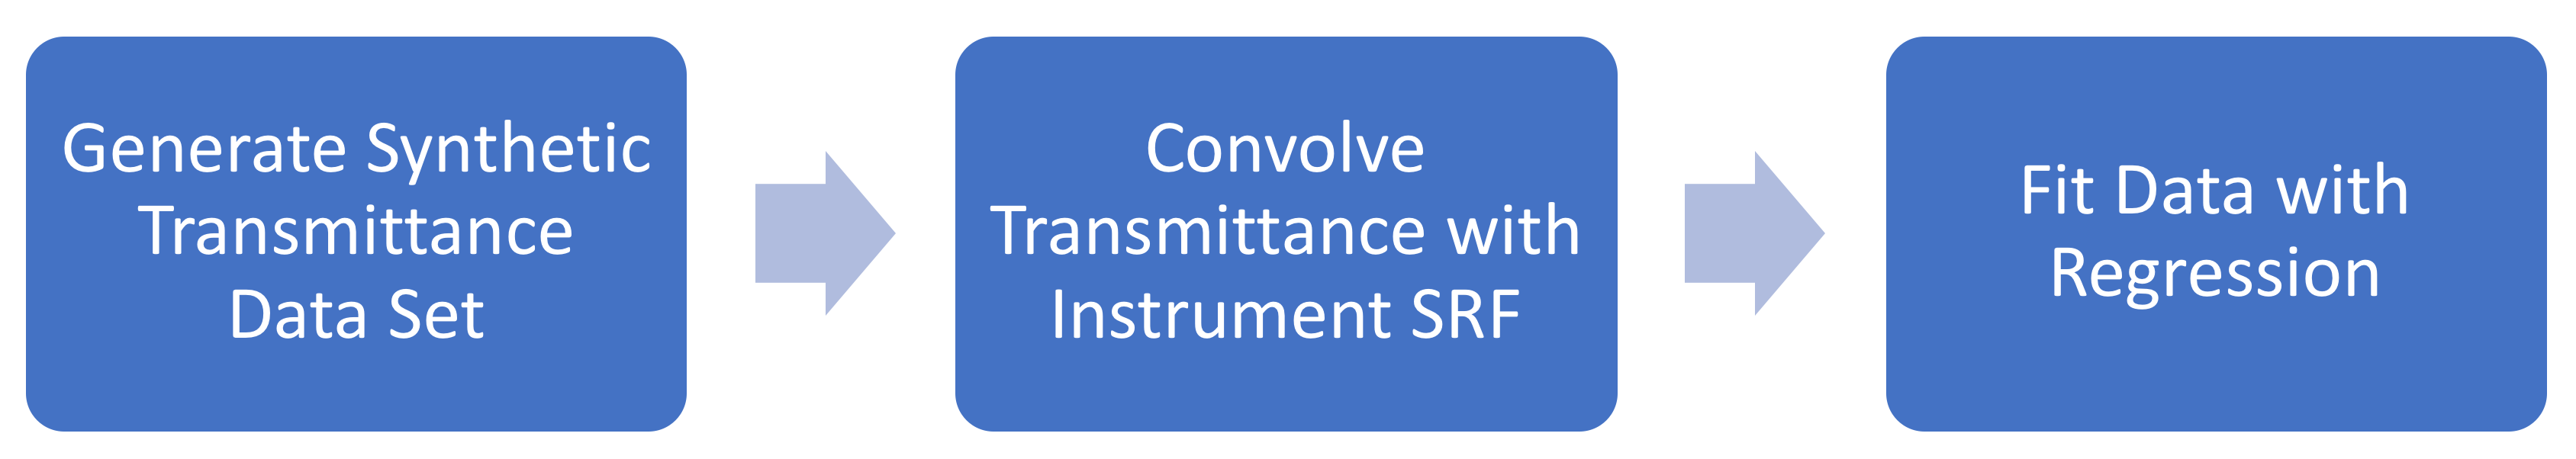
\includegraphics[width=1.\textwidth]{graphics/process_overview_1}
 \caption{High-level process overview.}
 \label{fig:proc1}
\end{figure}
As such, the high-level process is fairly straightforward and easy to grasp. First, a synthetic dataset of predictors and predictands needs to be generated. Second, a regression algorithm is used to find a simplified parameterization of the physical process that minimizes some definition of error, such as \emph{least-squares}. So the process has only two simple steps:

\begin{enumerate}
\item Line-by-line calculation of the layer-to-space transmittances for a specific instrument.
\item Regression calculations to fit the data.
\end{enumerate}
 
In practice however the process is very complicated due to the large number of special cases, depending on the frequency range, the specific instrument type, and various other physical effects, such as Zeeman splitting and non-LTE absorption.
Infrared instruments require using LBLRTM for Step 1, whereas microwave sensors can use MonoRTM or the Rosenkranz model available in the repository.
Consequently this guide will make a fundamental distinction between infrared radiation on the one hand, and microwave radiation on the other.
 \begin{figure}[H]
 \centering
 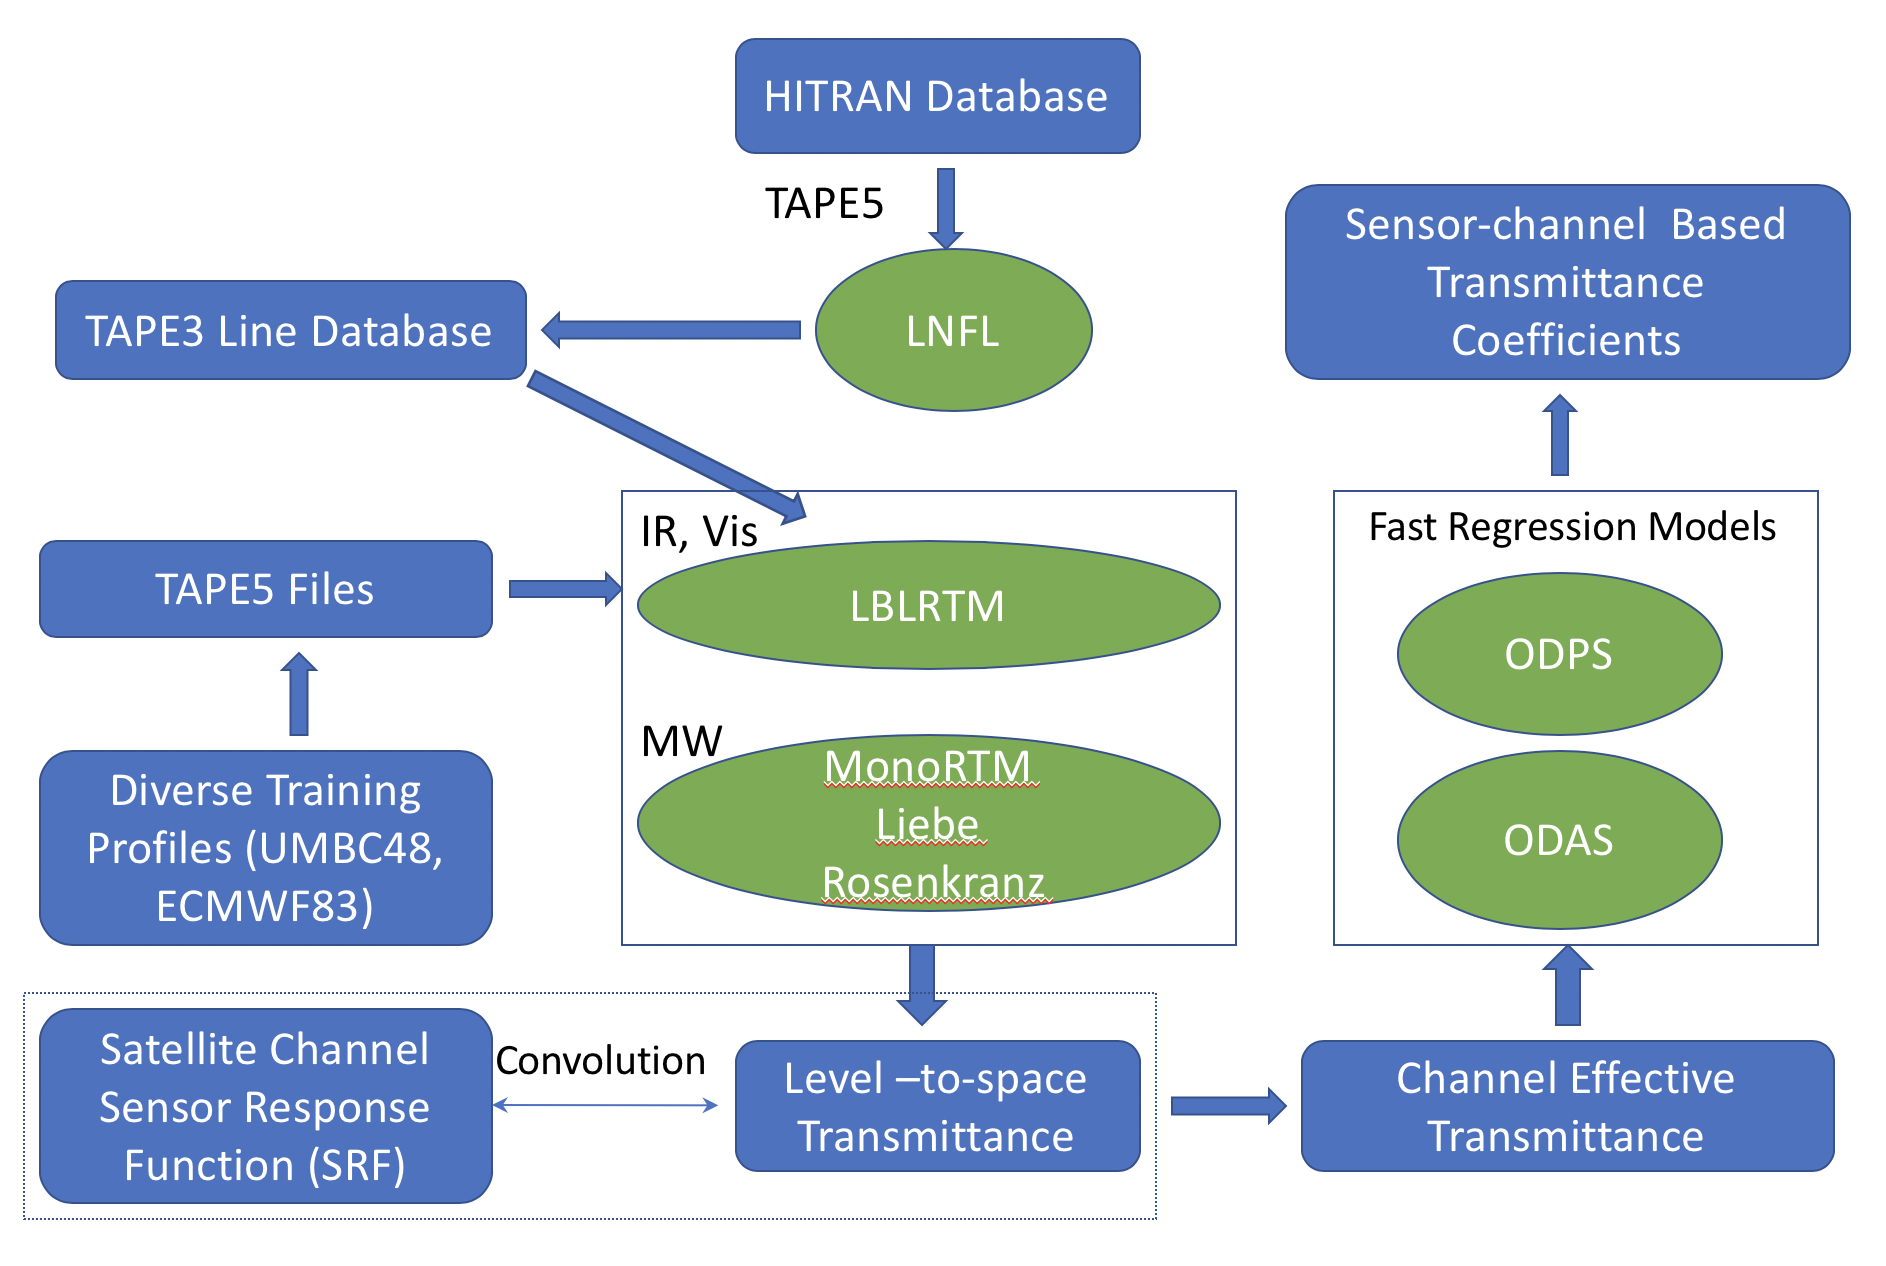
\includegraphics[width=1.\textwidth]{graphics/process_overview_2}
 \caption{Detailed coefficient generation process sketch.}
 \label{fig:proc2}
 \end{figure}

\section{Repository Overview}
The name of the Github repository is \verb CRTM_coef  and it consists of four basic folders;
\begin{itemize}
\item \begin{verbatim} src/ \end{verbatim}
\item \begin{verbatim} doc/ \end{verbatim}
\item \begin{verbatim} workdir/ \end{verbatim}
\item \begin{verbatim} cases/ \end{verbatim}
\end{itemize}
The first folder contains all the Fortran source code of this package, sorted by application. The folder is split into \verb TauProd  and \verb TauRegress  for Step 1 and Step 2 of the coefficient generation process, respectively.
Folder two contains the documentation pertaining to the package while the third folder, \verb workdir/  is for the convenience of the user and demonstrates a sample working directory for running all the steps of the coefficient generation process in one place. The working directory in turn contains two subfolders called \verb TauCoeffTest  and \verb GenCoeff . Their purpose is again to separate Step 1 and Step 2 of the process work. 
The last folder contains data for sample cases that are provided for validation purposes and that have been worked on during the package development.
 \begin{figure}[H]
 \centering
 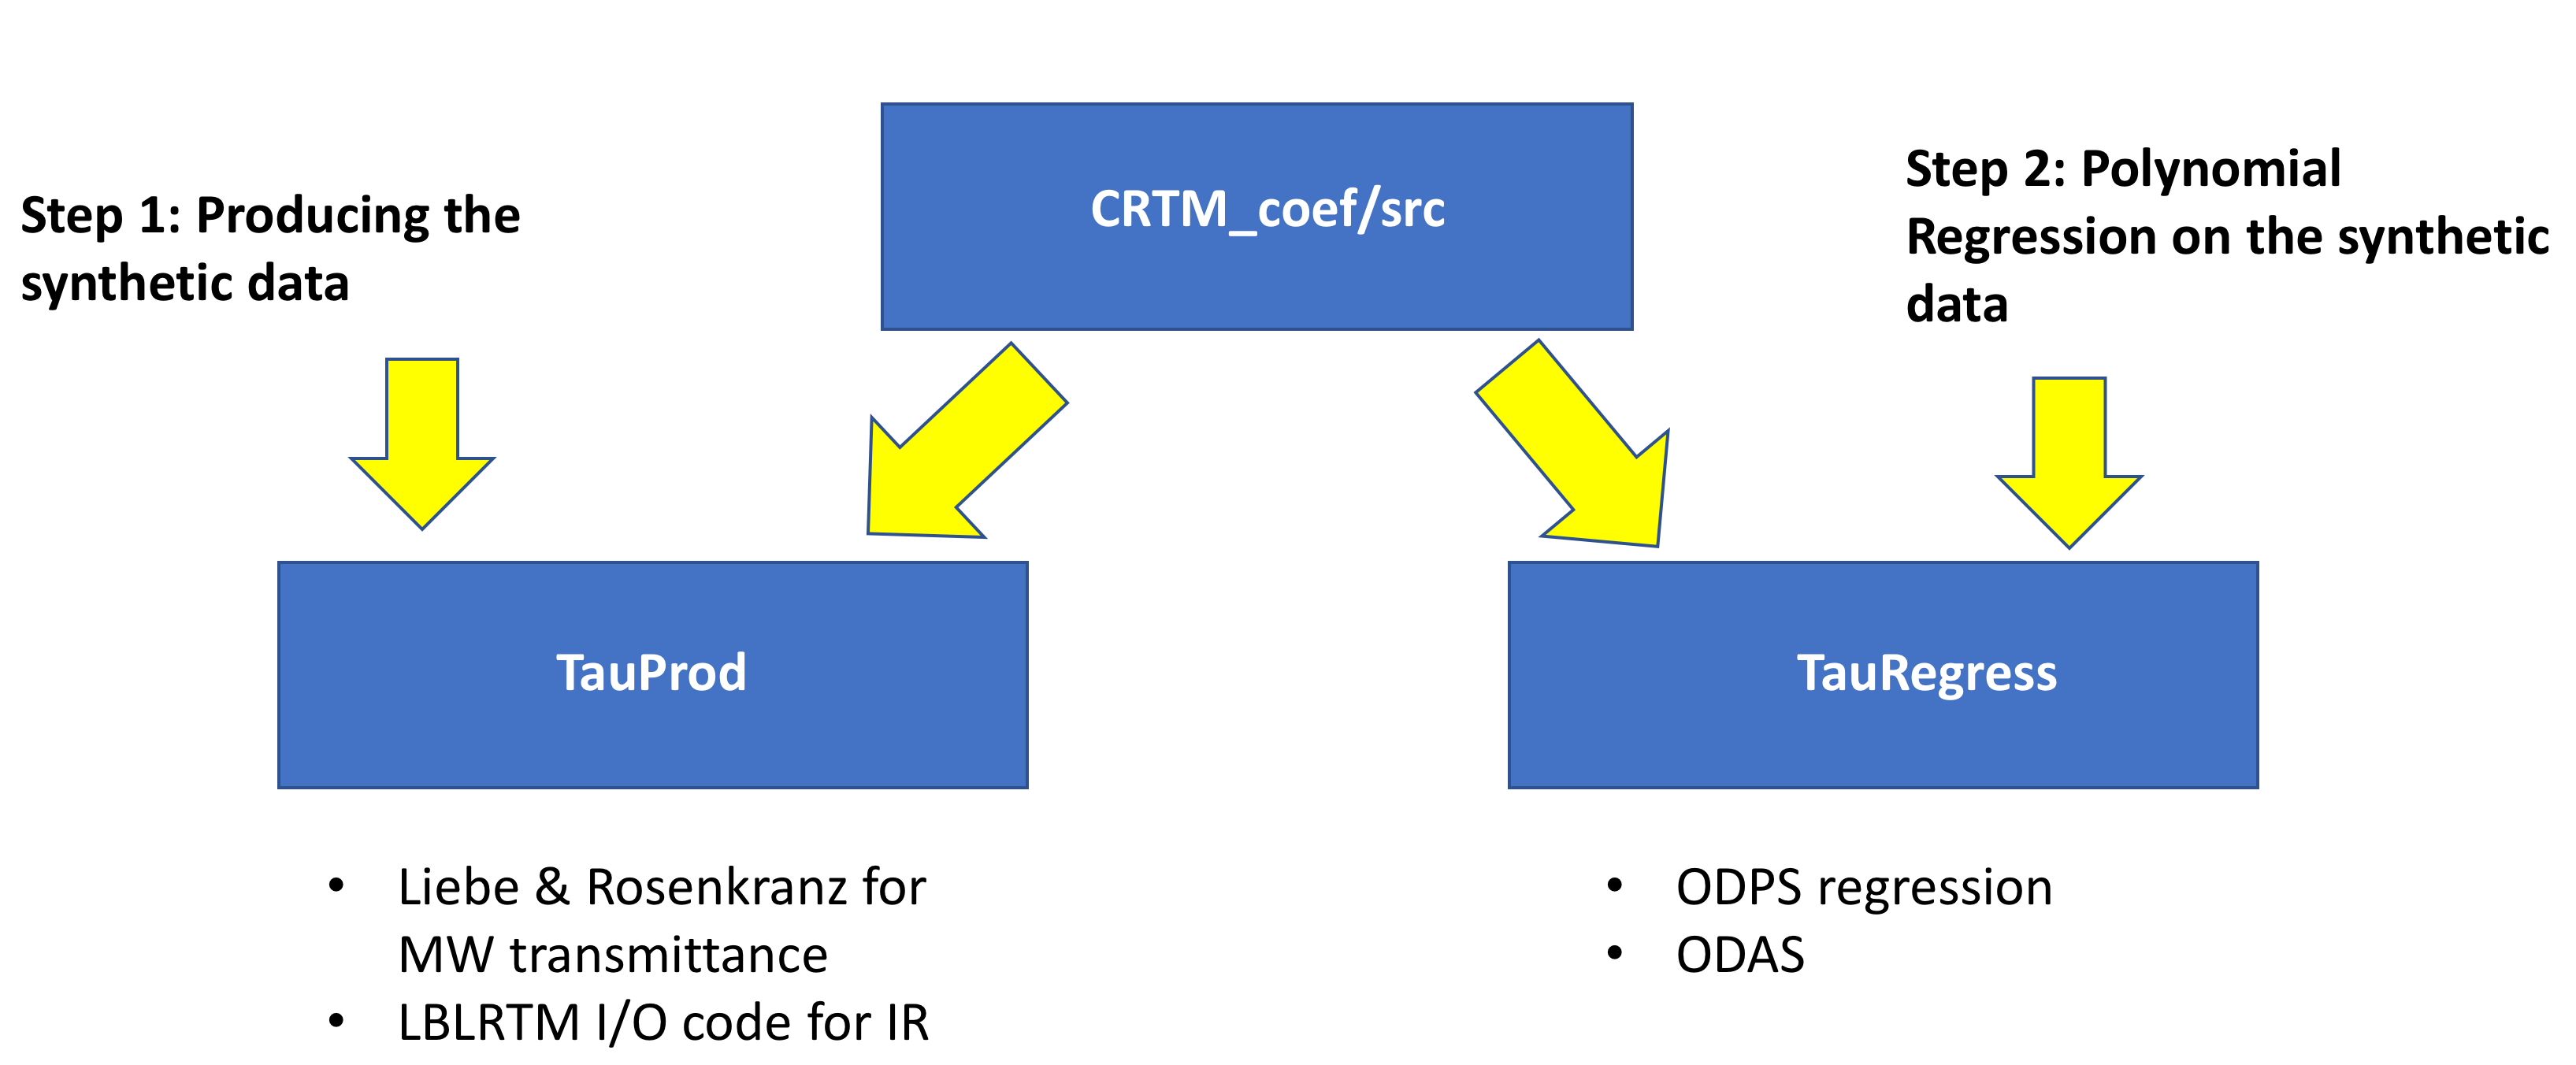
\includegraphics[width=1.\textwidth]{graphics/folder_structure}
 \caption{Repository structure.}
 \label{fig:foldstruct}
 \end{figure}

\section{How to compile the Code}
This section explains how to compile the code of the coefficient generation package. It provides details on how to obtain the required external support software and libraries, such as the codes from AER and the CRTM.

\subsection{Requirements}
\subsubsection{Supported Compilers}
First and foremost, this package requires a compatible Fortran compiler, as well as HDF5 and NetCDF4 file I/O libraries.
The package has been tested for the following Fortran compilers:
\begin{itemize}
\item Intel Fortran \verb ifort  (version 18.0.3 or higher)
\item GNU Fortran compiler \verb gfortran  (version 4.8 or higher)
\end{itemize}
and the following library versions:
\begin{itemize}
\item HDF5 (version 1.8 or higher)
\item NetCDF4 (version 4.6 or higher)
\end{itemize}

\subsubsection{Libraries maintained by the Joint Center}
Compiling the coefficient generation package requires two crucial libraries developed and maintained by the Joint Center for Satellite Data Assimilation:
\begin{itemize}
\item Community Radiative Transfer Model (CRTM) REL-2.1.3 or higher.
\item LBLRTMIO v0.1
\end{itemize}
Both these libraries are currently part of the \verb CRTM_dev  repository and should be cloned and compiled from the there.
Please see the corresponding user guides for both of these libraries \cite{lblrtmio,crtm} for instructions on how to compile, install, and link them properly.
LBLRTMIO can be found in the folder \verb CRTM_dev/src/TauProd/LBL/lblrtm  of the \verb CRTM_dev  repository. \textbf{It is important that you download and compile these aforementioned libraries successfully before you continue with this guide.}\\
The CRTM is required as the coefficient generation package relies on the same data structures that are implemented in the CRTM library. 
LBLRTMIO is a helper library to facilitate the otherwise tedious I/O communication with LBLRTM.

\subsubsection{External Software from AER}
The coefficient generation package also requires external software both from AER and the Joint Center for Satellite Data Assimilation. 
The codes from AER are in particular:
\begin{itemize}
\item LNFL v3.1 
\item LBLRTM v12.8
\end{itemize}
and optionally for microwave line-by-line calculations:
\begin{itemize}
\item MonoRTM v5.4 (this is currently not supported)
\end{itemize}

and the corresponding AER version of the \emph{HITRAN} database, \verb aer_3.6  . It is not necessary to obtain and compile this software before you begin compiling the code in the CRTM transmittance coefficient generation package. You will need these codes (except MonoRTM) before you can calculate a set of transmittance coefficients, however.

\subsection{How to Obtain and Compile LBLRTM}
In order to download these line-by-line models you will have to visit the AER website \url{http://rtweb.aer.com} and download the software from there. 
First, untar the downloaded archive:
\begin{verbatim}
$ untar xvf lblrtm_v12.8.tar
\end{verbatim}
Enter the directory of the LNFL application:
\begin{verbatim}
$ cd lblrtm_v12.8/lnfl
\end{verbatim}
Remove any executables that might potentially already exist, e.g.:
\begin{verbatim}
$ rm lnfl_v3.1_linux_intel_sgl
\end{verbatim}
then move to the \verb build  subdirectory and (re-) compile the LNFL application matching your architecture and compiler:
\begin{verbatim}
$ cd build/
$ make -f make_lnfl linuxGNUsgl
\end{verbatim}
A list of available compilation options can be found in the \verb README.build_instructions  file.
If the compilation process was successful, an executable called \verb lnfl_v3.1_linux_intel_sgl  should appear.
Now the same process needs to be repeated for the LBLRTM executable. 
Enter the lblrtm directory, remove the existing executable and *mod* files, and compile LBLRTM:
\begin{verbatim}
$ cd ../../lblrtm/
$ rm *mod*
$ make -f make_lblrtm linuxINTELdbl
\end{verbatim}
Then move to the \verb bin  directory, and create a softlink in this location with the executable that was just created:
\begin{verbatim}
$ cd ../bin
$ rm lblrtm
$ ln -s ../lblrtm_v12.8_linux_intel_dbl lblrtm
\end{verbatim}
In order to add LBLRTM to your path, you need to include the LBLRTM executable in your \verb .bashrc  file.

\subsection*{A note on running LBLRTM as a standalone model}
Running LBLRTM requires a \verb TAPE5  ASCII file that specifies the atmospheric state in terms of a profile of thermodynamic and trace gas variables and a \verb TAPE3  binary file that contains the spectroscopic line data. The \verb TAPE3  file is created by the LNFL application prior to running LBLRTM using an ASCII input file that is also called \verb TAPE5 , which is completely different from the LBLRTM \verb TAPE5  file, however.
In order to create a \verb TAPE3  file, you need to enter the \verb line_file  subdirectory, remove the existing \verb TAPE3  and run LNFL for the \verb TAPE5  configuration of your choice (examples can be found in the LBLRTM tutorial cases):
\begin{verbatim}
$ cd aer_v_3.6/line_file/
$ rm TAPE3.10-3500cm-1.*
$ ../../lnfl/lnfl_v3.1_linux_intel_sgl
$ mv TAPE3 TAPE.10-3500cm-1.first_7_molecules_reject
$ rm TAPE6 TAPE7 TAPE10
\end{verbatim}
Subsequently you may run LBLRTM via the \verb lblrun  utility script (or directly):
\begin{verbatim}
$ lblrun TAPE5 lblOutputFolderName
\end{verbatim}

\subsection{How to Compile the Coefficient Generation Code}
Care has been taken to simplify the considerable effort of compiling the individual executables of the coefficient generation package as much as possible. However, in the current configuration of the package there is currently no alternative to entering individual directories and compiling each executable in \verb src/  by hand.
\subsubsection{Compilation Macros}
A number of \verb make  macros have been defined in the repository root directory for a variety of systems. In order to use the macros for your particular system, please delete the existing \verb make.macros  and link the file with the ending corresponding to your system, e.g. for the S4 system:
\begin{verbatim}
$ rm make.macros
$ ln -s make.macros.s4 make.macros
\end{verbatim}

\subsubsection{Compiling the Fortran Source}
In order to compile the Fortran source code of the package, you need to enter the \verb CRTM_coef/src  directory and subsequently the individual application directory. 
Each specific task in the CRTM coefficient generation package is handled by exactly one Fortran application. The individual applications are connected via shell scripts.
In order to compile the code that generates TAPE5 input files as a simple example, you need to enter the corresponding directory and type \verb make  .
\begin{verbatim}
$ cd src/TauProd/AtmProfile/AtmProfile_Create
$ make -f Makefile
\end{verbatim}
This is a list of the individual applications in \verb src/  and their purpose:\\
%\begin{table}[H]
%\centering
\begin{center}
\begin{longtable}{ p{0.45\textwidth} | p{0.45\textwidth}}
  Folder Name: & Application Purpose:  \\ \hline
  \verb TauProd/AtmProfile/AtmProfile_Create/ & Creating NetCDF Atmospheric Profile files\\
  \verb TauProd/Infrared/ & \\
  \verb -"-/Assemble_TauProfile_Data & Assemble spectral layer-to-space NetCDF files\\
  \verb -"-/CheckProcessControl_File & Program to read a ProcessControl file to determine which channels have already been processed in the IR case\\
  \verb -"-/Compute_Effective_TauProfile & Program to compute effective layer-to-space transmittance data\\
  \verb -"-/Convolve_TauSpc & Duplicate copy of \verb Convolve_TauSpc_with_SRF  from CRTM trunk \\
  \verb -"-/Convolve_TauSpc_with_SRF & Convolve the monochromatic layer-to-space transmittance with the SRF\\
  \verb -"-/Create_LBLRTM_Input_Files & Creating \verb TAPE5  LBLRTM input files\\
  \verb -"-/Create_ProcessControl_File & Create a ProcessControl file for the convolution step\\
  \verb -"-/Create_Process_Defaults_File & Programm to create the defaults file for the IR process from the data specified in \verb Tau_Production_Parameters.f90 \\
  \verb -"-/Effective_TauProfile & \\
  \verb -"-/LBLRTM_to_netCDF & Convert the \verb TAPE20  binary output files from LBLRTM to NetCDF \\
  \verb TauProd/Microwave/ & \\
  \verb -"-/Compute_MW_Transmittance & Using the \emph{Liebe} or \emph{Rosenkranz} models to compute MW LBL transmittances\\
  \verb -"-/MW_TauProfile & Creating spectral microwave TauProfile datafiles based on oSRF inputs\\
  \verb TauRegress/ODAS/ & \\
  \verb -"-/Assemble_ODAS & Concatenate two ODAS TauCoeff files in netCDF format to a third file \\
  \verb -"-/ODAS_NC2BIN & Convert the ODAS NetCDF output into CRTM binary format \\
  \verb -"-/ODAS_Regress & ODAS regression code\\
  \verb TauRegress/ODPS/ & \\
  \verb -"-/Assemble_ODPS & Concatenate two ODPS TauCoeff files in netCDF format to a third file\\
  \verb -"-/GetSenInfo & Reading sensor info from file\\
  \verb -"-/ODAS_WLO_Regress & ODAS water vapor line regression code for merging with ODPS \\
  \verb -"-/ODPS_NC2BIN & Converting ODPS NetCDF output to CRTM binary format \\
  \verb -"-/ODPS_Regress & ODPS regression code \\
  \caption{List of folders in the package and their purpose.}
  \label{tab:folders}
\end{longtable}
\end{center}
%\end{table}
Please reference this list \ref{tab:folders} when following the coefficient generation process workflow.

\subsubsection*{Common Compilation Issues}
There are a number of common issues that you may encounter when trying to compile the source code. The list here is by no means exhaustive, but it is meant as a starting point for any debugging efforts.

\paragraph{The HDF5 or NetCDF4 libraries are not linked correctly}
Using the package on an unsupported machine may lead to libraries not being found during the linking step.
In this case you will need to modify the makefiles according to your own setup. Generally the makefiles will contain the following sequence, which you will need to modify:
\begin{verbatim}
NC4_DIR=/opt/netcdf4/4.6.2-intel-18.0.3
HDF_DIR=/opt/hdf5/1.8.21-intel-18.0.3
HDF4_DIR=/opt/hdf4/4.2.14-intel-18.0.3

INCLUDES = -I$(NC4_DIR)/include -I$HDF_DIR)/include

LIBRARIES = -L$(NC4_DIR)/lib -lnetcdf -lnetcdff  -L$(HDF_DIR)/lib -lhdf5
\end{verbatim}


\paragraph{LBLRTMIO is not linked correctly}
As you need to compile the LBLRTMIO on your own, it is likely that it will not be linked correctly.
In general, an application that uses LBLRTMIO should contain the following lines:
\begin{verbatim}
# Compilation flags
EXTRA_FC_FLAGS = -I$(CRTM_PATH)/src/TauProd/LBL/lblrtm/build/libsrc/include

# Linking flags
LIBRARIES = -L$(CRTM_PATH)/src/TauProd/LBL/lblrtm/build/libsrc/lib -llblrtmio
\end{verbatim}
These should be modified in case LBLRTMIO is not linked correctly.

\section{How to generate New Coefficients}
The guide on how to generate new CRTM transmittance coefficients follows the distinction outlined in the introduction: \textbf{Step 1:} \emph{TauProd} and \textbf{Step 2:} \emph{TauRegress}.

\subsection{TauProd: Line-by-Line Transmittance Calculations}
Physically rigorous computations of gaseous transmittance in the atmosphere require so-called line-by-line radiative transfer models that are based on resolving all gas absorption lines in a given spectral window. As these models require too many computational resources they are currently impractical for data assimilation applications.
However, their rigorous treatment of the absorption process makes it possible to use them as a basis for developing fast models and their results are usually considered as \emph{"exact"} in this context.\\
\begin{figure}[H]
 \centering
 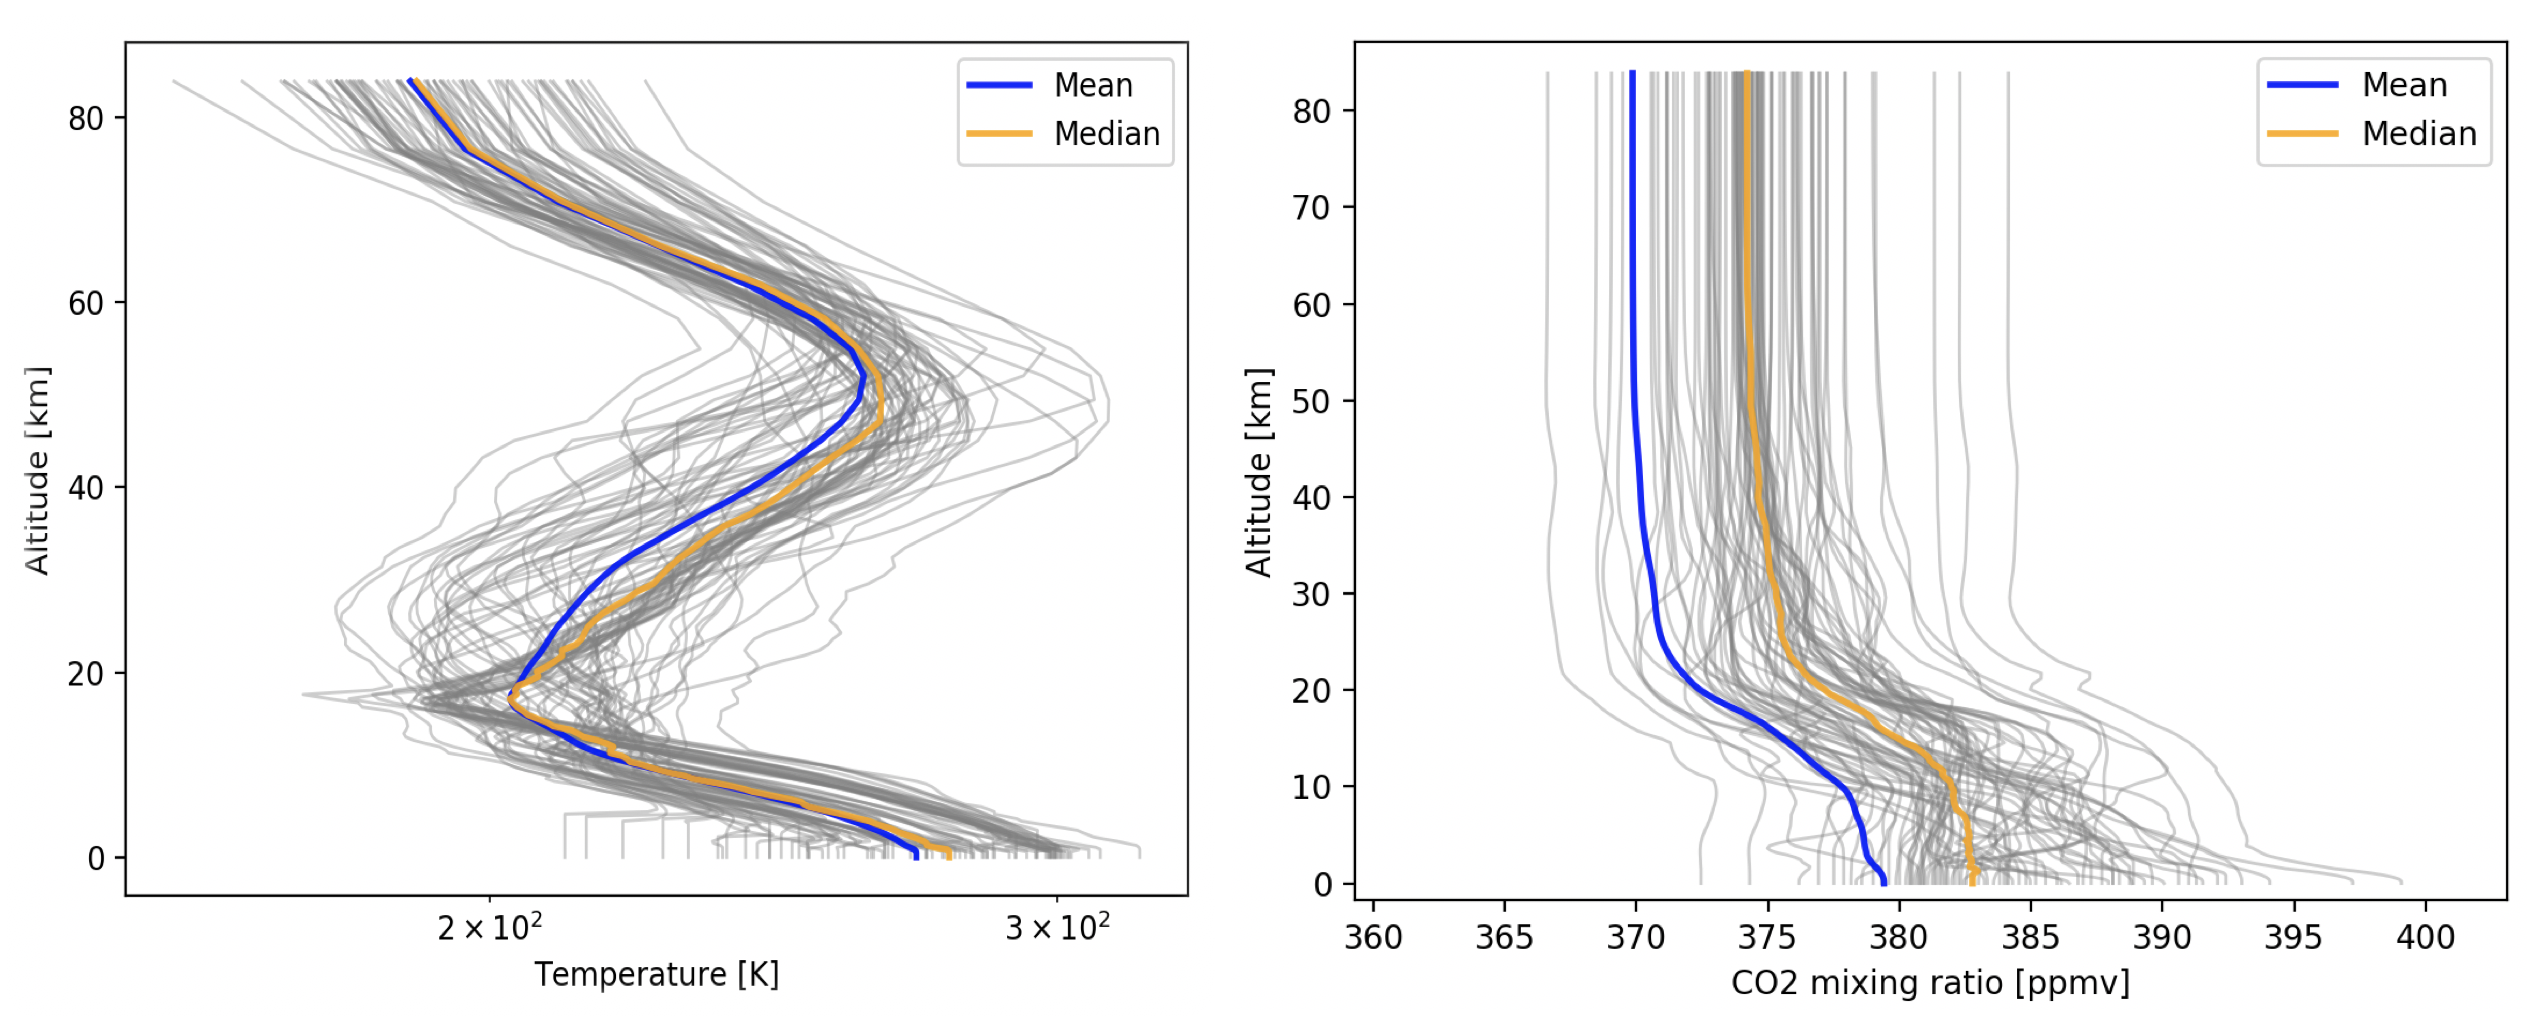
\includegraphics[width=1.\textwidth]{graphics/ECMWF83_profiles_pic}
 \caption{ECMWF83 predictor data set.}
 \label{fig:prof}
 \end{figure}
This subsection provides a description on how to perform line-by-line calculations for the CRTM both in the MW and the IR region. It should be noted that the microwave process is considerable less involved than the infrared process which requires using LBLRTM.
The computed line-by-line layer-to-space transmittances in the infrared case also require considerably more storage space and the infrared computations are generally only possible on a cluster, while the microwave computations can be conveniently performed on a laptop.

\subsubsection{Microwave}
The line-by-line calculations for microwave instruments are fairly straightforward and can be performed on a laptop, as they are based on a CRTM-internal implementation of the \emph{Liebe89} and \emph{Rosenkranz03} transmittance models.\\
Performing the calculations requires the following steps:
\begin{enumerate}
\item Enter the directory \verb src/TauProd/Microwave/MW_TauProfile/ .
\item Compile the code in the folder by typing \verb make .
\item Link in the atmospheric training profile, e.g. for the ECMWF83 set: 
\begin{verbatim}
$ ln - s fix/ECMWF83.AtmProfile.nc ./ 
\end{verbatim}
\item Link in the instrument oSRF file, e.g. for AMSU-A:
\begin{verbatim}
$ ln -s fix/amsua_n15.osrf.nc ./
\end{verbatim}
\item Link in the SensorInfo file e.g.:
\begin{verbatim}
$ ln -s cases/amsua_metop-c_benchmark/SensorInfo-amusa_metop-c ./
\end{verbatim}
\item Run the \verb MW_TauProfile  executable and follow the prompted instructions based on the linked data and files.
\end{enumerate}
In case of a successful computation the spectral layer-to-space NetCDF output file will appear with the generic name \verb upwelling.<sensor_name>.TauProfile.nc . This file provides the basis for the subsequent regression algorithms (either ODAS or ODPS).

\subsubsection{Infrared}
The infrared line-by-line calculations require a working version of LBLRTM v12.8 or higher and access to a cluster computing environment.
In order to start the process you first need to enter the \verb TauCoeffTest  directory and continue the process from there:
\begin{verbatim}
$ cd workdir/IR/TauCoeffTest/
\end{verbatim}

\paragraph{Creating TAPE3 input files} 
LBLRTM requires \verb TAPE3  files as an input. These files contain the absorption line parameters for the selected absorbers in binary format.
In order to create \verb TAPE3  files, enter the \verb lnfl/  directory and run the \verb ./run_lnfl  script:
\begin{verbatim}
$ cd lnfl/
$ ./run_lnfl
\end{verbatim}
This creates the basic \verb TAPE3  templates for the IR LBLRTM calculations.

\paragraph{Creating TAPE5 input files} 
The other necessary input for LBLRTM is the atmospheric profile in terms of a \verb TAPE5 file. The \verb TauCoeffTest  folder already contains \verb TAPE5  files for the ECMWF83 profile set. 
In case you want to try a different profile set you need to translate the NetCDF input profile set into a set of \verb TAPE5  files via the \verb Create_LBLRTM_Input_Files  application:
\begin{verbatim}
$ cd src/TauProd/Infrared/Create_LBLRTM_Input_Files	# Enter the folder
$ make 										# Compile the application
$ ./Create_LBLRTM_Input_Files					# Follow the prompted instructions
\end{verbatim}
After successful completion of this step, enter the \verb TAPE5_files  folder that contains the produced \verb TAPE5  files and run the \verb attach_scnmrg_suffix  shell script to append the instruction set to all \verb TAPE5  that instructs LBLRTM to produce the \verb TAPE20  output that contains the required layer-to-space monochromatic transmittances:
\begin{verbatim}
$ cd TAPE5_files
$ ./attach_scnmrg_suffix
\end{verbatim}
As a final step, link the produced \verb TAPE5  files into the \verb TauCoeffTest  folder.
\begin{verbatim}
$ cd ..
$ ln -s TAPE5_files/ workdir/IR/TauCoeffTest/
\end{verbatim}

\paragraph{Preparation of the working directory}
The preceding two steps have shown how to prepare the \verb TAPE3  and \verb TAPE5  input files for the LBLRTM calculations. The subsequent preparation steps have largely already been carried out in the example \verb workdir/  of the \verb CRTM_coef  repository and are listed here to enable the users to setup their own line-by-line calculations.\\
In order to setup the working directory, the following steps need to be taken:
\begin{enumerate}
\item Link in the oSRF of your instrument in the subdirectory \verb TauCoeffTest/oSRF_Data .
\item Link the \verb SensorInfo file into \verb TauCoeffTest .
\item Ensure that the \verb TAPE5  files are linked into the working directory.
\item Create a subdirectory \verb TauProfile_data  and link \verb SensorInfo  into it.
\end{enumerate}

\paragraph{Configuration}
Before starting the LBLRTM calculations you need to prepare a \emph{"TauProd defaults file"} called \verb Transmittance_Production.processing_defaults . An example file of this type is already provided in the \verb TauCoefftest  folder and you may modify it as you see fit.
This file specifies the parameters for the LBLRTM run. A collection of these parameters is unfortunately also hard-coded in the \verb Tau_Production_Parameters.f90  Fortran source file. An alternative to modifying the provided \verb Transmittance_Production.processing_defaults  file is to run the \verb Create_Process_Defaults_File  application that produces such a file based on the hard-coded parameters in \verb Tau_Production_Parameters.f90 .
A typical for an ODAS run looks like this:
\begin{verbatim}
:QUEUE:serial:Default batch processing queue
:BAND1:1:Beginning band to process
:BAND2:13:Ending band to process
:F1_BAND1:500:The begin frequency of band #1
:DF_BAND:250:The effective bandwidth of each band
:DF_AVG:0.1000:The averaging kernel frequency width. Must have 4dp
:DF_INDEX:2:The averaging kernel frequency width index
:TAPE3_LIST:1 10 11 12 13 14 15:Molecule set numbers
:TAPE3_ID:aer_v_3.6:The spectroscopic database to use
:TAPE5_DIR:./TAPE5_files:The directory where the TAPE5 files are located.
:PROFILE1:1:Beginning profile to process
:PROFILE2:83:Ending profile to process
:PROFILE_SET_ID:ECMWF83:Profile set identifier
:PROFILE_SET_NUMBER:5:Profile set identifier number
:ANGLE1:1:Beginning angle to process
:ANGLE2:7:Ending angle to process
\end{verbatim}
while a typical file for an ODPS run looks like this:
\begin{verbatim}
:QUEUE:serial:Default batch processing queue
:BAND1:64:Beginning band to process
:BAND2:90:Ending band to process
:F1_BAND1:500:The begin frequency of band #1
:DF_BAND:25:The effective bandwidth of each band
:DF_AVG:0.0025:The averaging kernel frequency width. Must have 4dp
:DF_INDEX:2:The averaging kernel frequency width index
:TAPE3_LIST:7 10 15 18 19 20 21 22:Molecule set numbers
:TAPE3_ID:aer_v_3.6:The spectroscopic database to use
:TAPE5_DIR:./TAPE5_files:The directory where the TAPE5 files are located.
:PROFILE1:1:Beginning profile to process
:PROFILE2:83:Ending profile to process
:PROFILE_SET_ID:ECMWF83:Profile set identifier
:PROFILE_SET_NUMBER:5:Profile set identifier number
:ANGLE1:1:Beginning angle to process
:ANGLE2:7:Ending angle to process
\end{verbatim}
It is possible to deviate from these parameters to include e.g. a custom frequency range or absorber combination, however this will currently still lead to problems further down the road in the process with the convolution and regression steps.

\paragraph{Submitting the TAPE5 jobs}
After the setup step is complete, the LBLRTM calculations can start by submitting the driver script to the \emph{serial} queue of a \verb slurm  scheduler:
\begin{verbatim}
$ sbatch ./submit_process_tape5
\end{verbatim}
\textbf{\textcolor{red}{Warning:}} This step will create a large number of folders in the working directory, one for each band, absorber combination, and viewing angle. 

\paragraph{The SRF Convolution Step}
In order to convolve the monochromatic transmittance profiles with the instrument SRF, submit the \verb submit_process_TauSpc  script to the serial queue of a \verb slurm  scheduler:
\begin{verbatim}
$ sbatch ./submit_process_TauSpc
\end{verbatim}
This script submits the \verb process_TauSpc_files  shell script. Please ensure that all application locations in the header of \verb process_TauSpc_files  are set correctly and that the variable \verb DF_INDEX  is set to the correct frequency-delta index that is also used in the instrument oSRF file and the \verb Transmittance_Production.processing_defaults  file. The range of values can be 1, 2, or 3.

\paragraph{Concatenating the Spectral Transmittance Profiles}
In order to combine all individual spectral transmittance profiles into a single one, create a \verb pc.generic  configuration file and run the \verb process_TauProfile_files  shell script. To this end you may either run the \verb Create_ProcessControl_File , or link an existing \verb pc.generic  file from one of the computation folders:
So you need to either do the following:
\begin{verbatim}
$ cd src/TauProd/Infrared/Create_ProcessControl_File/
$ ./Create_ProcessControl_File
\end{verbatim}
or the following:
\begin{verbatim}
$ ln -s profile01/angle1/mol1/ProcessControl.angle1_mol1.upwelling pc.generic
\end{verbatim}
Subsequently you can run the \verb process_TauProfile_files  shell script:
\begin{verbatim}
$ ./process_TauProfile_files -d up
\end{verbatim}
This step concludes the LBLRTM computation process and you can move on to the regression.

\subsection{TauRegress: Statistical Regression}
This section is focused on the \textbf{ODPS} regression algorithm alone. The default working directory for the IR regression is \verb workdir/IR/GenCoeff .
\begin{verbatim}
$ cd workdir/Infrared/GenCoeff/
\end{verbatim}
In the \verb GenCoeff/  directory you will find the \verb sensor_list  file. This file contains the \emph{sensor id} of the instruments for which the regression should be performed.
In order to run the regression, please add the \emph{sensor id} to the \verb sensor_list  file, e.g. for AVHRR3:
\begin{verbatim}
## This file contains a list of sensors and is one of the input file of
## run_gensub.sh
## Only those between BEGIN and END are processed.

BEGIN_LIST
avhrr3_n19
END_LIST
\end{verbatim}

Edit the \verb taucoeff.parameters  configuration file to point to the correct absolute path of the required executables and working directory. An example is provided in the \verb GenCoeff/  directory. Please modify it accordingly.
Finally, run the \verb run_tau_coeff.sh  shell script. As you can see below, you will need to run the first three of the four provided steps in order by uncommenting the respective line. 
The fourth step is currently not functional.
\begin{verbatim}
#!/bin/sh

#------------------------------------------------------------------------
# Generate transmittance coefficients for each channel and tau component
#------------------------------------------------------------------------

#-----------------------------------
# 1): Generate tau coefficients
#-----------------------------------

./gen_tau_coeff.sh tau_coeff.parameters

#------------------------------------------------------------------
# 2) Get fitting errors for each component - run after 1)
#------------------------------------------------------------------

#get_stat.sh tau_coeff.parameters

#----------------------------------------------------------------------
# 3) Merge (concatenate) tau coefficient files into one - run after 1)
#----------------------------------------------------------------------

#EXE_file=../../../src/TauRegress/ODPS/Assemble_ODPS/Cat_ODPS
#./cat_taucoef.sh tau_coeff.parameters $EXE_file

#-----------------------------------------------------------------------------
# 4) Compute fitting error for each channel (all component) - run after 1) & 3)
#-----------------------------------------------------------------------------

#EXE_file=../src_FitErr/Compute_FitErr
#EXE_file=/jcsda/save/wx23yc/CRTM_ODPStraining/training/src_FitErr/Compute_FitErr
#set it to 1 to include OPTRAN wlo and set it to 0 to exclude it
#OPTRAN=1
#run_Compute_FitErr.sh tau_coeff.parameters $EXE_file $OPTRAN

exit

\end{verbatim}

This concludes the transmittance coefficient training process. The final coefficient file will be available in NetCDF format and can be converted to CRTM native format using one of the utility programs, such as\\ \verb src/TauRegress/ODPS/ODPS_NC2BIN .

% The references section
%=======================
\clearpage
\bibliographystyle{plainnat}
\bibliography{bibliography}

\begin{thebibliography}{9}

\bibitem{yongchen}
  Yong Chen, Yong Han, Paul Van Delst, and Fuzhong Weng
  \textit{ On water vapor Jacobian in fast radiative transfer model (sic)},
  J. Geophys. Res.,
  115 D12303,
  2010.
  
\bibitem{optran}
  Larry McMillin, and Henry Fleming,
  \textit{ Atmospheric transmittance of an absorbing gas: a computationally fast and accurate transmittance model for absorbing gases with constant mixing ratios in inhomogeneous atmospheres},
  Applied Optics,
  15(2) 358-363,
  1976. 
  
\bibitem{rttov}
  Marco Matricardi
  \textit{The generation of RTTOV regression coefficients for IASI and AIRS using a new profile training set and a new line-by-line database},
  ECMWF Research Department,
  Technical Memorandum,
  2008. 

\bibitem{lblrtmio}
  Paul van Delst
  \textit{LBLRTMIO v0.1 User Guide},
   Joint Center for Satellite Data Assimilation,
  Technical Memorandum,
  2004. 
  
  \bibitem{crtm}
  Paul van Delst
  \textit{CRTM REL-2.1.3 User Guide},
  Joint Center for Satellite Data Assimilation,
  Technical Memorandum,
  2004. 

\end{thebibliography}

\newpage

% The appendices section
%=======================
\begin{appendix}
\section*{Appendix}
\section{SCNMRG  suffix template for TAPE5 }
At the end of a regular \verb TAPE5  file a suffix has to be attached to instruct LBLRTM to produce output in \verb TAPE20  format.
If this sequence is not attached the LBLRTM calculation will still finish successfully, but the output will not be in the required format.
\begin{verbatim}
$ SCNMRG of precalculated KODFILS upwelling -> TAPE20
 HI=0 F4=0 CN=0 AE=0 EM=0 SC=0 FI=0 PL=0 TS=0 AT=0 M=35 LS=0 MS=0 XS=0    0    0
ODdeflt_                                                 100
    C.CCCC SSSS.SSSS TTTT.TTTT    0    0    0   -D.DDDD                  20    5
0.00000000
$ SCNMRG of precalculated KODFILS downwelling -> TAPE21
 HI=0 F4=0 CN=0 AE=0 EM=0 SC=0 FI=0 PL=0 TS=0 AT=0 M=36 LS=0 MS=0 XS=0    0    0
ODdeflt_                                                 100
    C.CCCC SSSS.SSSS TTTT.TTTT    0    0    0   -D.DDDD                  21    5
0.00000000
%
\end{verbatim}
Note that character values such as \verb TTTT.TTTT  are template parameters that are later replaced with floating point frequency values when calling the \verb proces_tape5_files  shell script.

\section{List of known Error Messages}
This section contains a list of known errors together with suggested solutions.
The errors are sorted by the workflow step in which they may be encountered.

\subsection{Compile Phase}

\subsection{Line-by-line Phase}

\subsection{SRF Convolution Phase}
\paragraph{Error Message:}
\begin{verbatim}
 Create_ProcessControl_File(FAILURE) : Invalid frequency interval,  
 1.000000E-01cm^-1, detected for channel
 ...
 Convolve_TauSpc(FAILURE) : Different dF_Index values in 
 ProcessControl file ProcessControl.angle1_wco.upwelling
\end{verbatim}
\paragraph{Solution:}
The \verb DF_INDEX  of the LBLRTM calculation bands and the \verb Frequency  grid data in the instrument oSRF file do not match.
Consequently the LBLRTM calculations need to be repeated with the correct \verb DF_INDEX  value. 

\subsection{Regression Phase}

\end{appendix}

\end{document}

